\chapter{Used methods and algorithms}

In previous chapter I have introduced you to several kinds of agents, how they can be used and also what a spatial memory is. I have briefly prepaired you for the next chapters, where I will explain my contribution to this area. This chapter is going to cover the used algorithms and computational methods I have studied and implemented in my work. 

The first subsection disserts on the implementations of agents' memory and in detail describes fundamental parts. Both the Growing Neural Gas and the Quad..blah are used as memory storages to handle spatial information about the environment with bounded resources.

\section{Growing Neural Gas}   
\label{usedalgo:gng}

\subsection{Topology learning}

Processing an enormous spatial data about an environment is computationaly demanding when for example we want to navigate in that environment. A topology learning or recognition can help us to create a representation such as topological map which can be viewed as a graph and which makes reasoning in that environment much easier. Rather complex understanding of topology in an indoor space using Bayesian programming has been shown in \cite{Tapus:topologylearning}. It goes much farther than I need to. 

Based on competitive Hebbian learning (CHL) method \cite{Martinetz:chl} and Neural Gas (NG) \cite{Martinetz:ng} Bern Fritzke suggested earlier mentioned Growing Neural Gas \cite{Fritzke:gng}, an unsupervised learning method for finding a topological structure which reflects the topology of the data distribution. Although the combination of both CHL and NG is an effective method for topology learning, there are some flaws in practical application as it requires an initial setup of number of nodes/centers that are used. This fact prevents the method from adequately describing the topology, when a different number of nodes would work better.

As Fritzke described the algorithm uses a set of nodes and edges that connects the nodes. A simplified describtion of algorithm from \cite{Fritzke:gng} in context of two-dimensional space follows:

\begin{enumerate}
\item Add two nodes at random position onto canvas
\item Generate input signal based on the data distribution (its probability density)
\item Find the nearest node $n_1$ and second nearest node $n_2$ to the signal
\item Increment the age of all edges leading from node $n_2$
\item Add the squared distance between the input signal and the nearest unit in
input space to a local counter variable $\Delta error(n_{1})$
\item Moved node $n_1$ and its topological neighbors towards the signal (according to parametres $epsilon_{winner}$ and $epsilon_{neighbour}$)
\item Remove all edges with an age larger than $a_{max}$
\item Generate new nodes (see \cite{Fritzke:gng}) using variable $alpha$
\item Decrease all error variables by multiplying them with a constant $beta$
\item Go to 1.
\end{enumerate}

For the purpose of this work I want to use this algorithm to learn a topology of data which dynamically changes through the time. We have to setup the variables for this agorithm $alpha$, $beta$, $epsilon_{winner}$, $epsilon_{neighbour}$ and maximal number of nodes. In following subsection I am going to introduce you to the experimenting with this algorithm.

\subsection{Experiments on dynamic data}

As I have mentioned previously I had to setup the variables so as to be able to use Growing Neural Gas method properly. To attain this goal I have made a Java programm which tests various combinations of variables' values and finds the best one. It has sequently run the algorithm for a given number of steps and measured the \emph{score} (see \ref{usedalgo:scoremethod}).

\begin{figure}
\begin{lstlisting}[language=Pascal]
procedure Score()
  (px, py, pvar) <- GetProbableGauss()
  (rx, ry, rvar) <- GetRealGauss()
  
  sqDistance <- (px - rx)*(px - rx) + (py - ry)*(py - ry)
  sqSize <- (pvar + rvar)*(pvar + rvar)
  
  score <- sqDistance / sqSize
  
  return score
end
\end{lstlisting}       
\caption{The \emph{SCORE} method}
\label{usedalgo:scoremethod}
\end{figure}
       
\begin{figure}      
\begin{center}
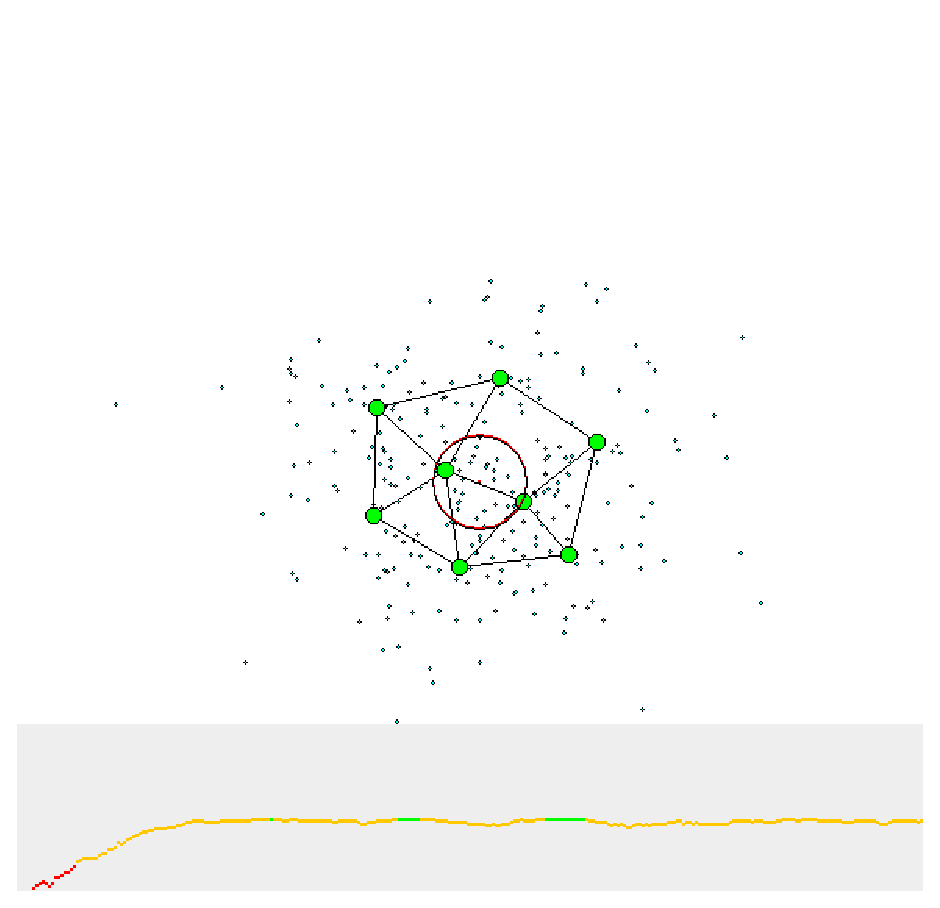
\includegraphics[scale=0.75]{images/gng/experimental_setup.eps}    
\caption{Screenshot showing the process of searching optimal variable values. The visualization has been made for testing purposes in the first place, but it nicely shows what had been lately paralelly computed. The bottom part of the picture shows the SCORE value throughout the simulation. {\emph (Red color means $SCORE > 0.05$, orange is $SCORE > 0.001$ and green is $SCORE <= 0.001$)} }
\end{center}                          
\label{usedalgo:gngexperimentscreen}
\end{figure}

\begin{figure}          
\begin{itemize}
\item $alpha \in \{0.0, 0.2, 0.4, 0.5, 0.6, 0.8, 1.0\}$
\item $beta \in \{0.0, 0.00001, 0.00005, 0.0001, 0.001, 0.005, 0.01, 0.5, 0.1, 0.5, 1.0\}$
\item $epsilon_{winner} \in \{0.0, 0.001, 0.005, 0.01, 0.1, 0.2, 0.5, 1.0\}$
\item $epsilon_{neighbour} \in \{0.0, 0.0001, 0.0006, 0.001, 0.005, 0.05, 0.1, 0.2\}$
\item $maxNodes \in \{4, 8, 16, 32\}$
\end{itemize}
\caption{Domains of variables for the experimental learning of best values.}
\label{usedalgo:gngexperimentdomains}
\end{figure}

A total number of possible combinations is equal to 19712. For each such a combination I have run 10000 steps of GNG learning sequence and measured the average score. Each sequence took aproximately 108 seconds and all the experiment was computed paralelly using 30 threads.

The best results which were avarage $SCORE < 10^{-11}$ is shown in a table \ref{usedalgo:gngexperimentresults}.

\begin{table}
\begin{center}
\begin{tabular}{ccccc|c}

$alpha$ & $beta$ & $epsilon_{winner}$ & $epsilon_{neighbour}$ & $numNodes$ & $SCORE$ \\
\hline
0.0 & 1.0 & 0.0050 & 0.0 & 16 & $3.8*10^{-12}$ \\
0.5 & 0.0 & 0.01 & 1.0E-4 & 8 & $5.1*10^{-12}$ \\   
0.5 & 0.0010 & 0.1 & 0.0010 & 8 & $8.8*10^{-12}$ \\ 
0.5 & 1.0 & 0.0 & 1.0E-4 & 8 & $3.1*10^{-12}$ \\     
0.8 & 1.0E-5 & 0.0010 & 1.0E-4 & 32 & $7.4*10^{-12}$ \\
0.8 & 1.0E-5 & 0.0050 & 6.0E-4 & 8 & $4.3*10^{-12}$ \\

\end{tabular}      
\caption{\label{usedalgo:gngexperimentresults}Variable values with best average SCOREs}
\end{center}
\end{table}

\section{Grid}
\label{sec:grid}

The idea for this data structure representing resource-bounded memory is based on \cite{Brom:placeandobjects}. What differs in my work from their observed environment is agents in my simulation act in a homogeneous space which cannot be differentiated in a way the mentioned simulation does. To solve this issue I have simply differentiated the environment into grid 4x4, where each cell works as the place in \cite{Brom:placeandobjects}. 

Each cell is given two variables {\emph positive} and {\emph negative} both of which are set to zero and increased throughout the simulation. When an agent sees at least half of that area determined by the cell, if he sees any food, he increase the {\emph positive} variable. If the agent search for food and he cannot see any, he increase the {\emph negative} variable.

When the grid is later asked whether there is food at specific cell, it answers according to this method with parametr $\alpha$ to be found:

\begin{equation} ANSWER = \alpha\times positive - negative 
\end{equation}
 
Similary I will use this structure to keep spatial information about the environment in the simulation.